\documentclass[11pt,runningheads,a4paper]{article}
\usepackage[utf8]{inputenc}
\usepackage{amsmath,amssymb,hyperref,array,xcolor,multicol,verbatim,mathpazo}
\usepackage[normalem]{ulem}
\usepackage[pdftex]{graphicx}
\usepackage{fullpage}
\usepackage{hyperref}
\usepackage{float}
\usepackage{listings}
\usepackage{romannum}
\begin{document}
%%%% In most cases you won't need to edit anything above this line %%%%

\title{{\LARGE Bioinformatics Supervision}\\
{\Large --Problem Sheet 2--}} 
\author{Supervisor: Sebastian Müller (Department of Plant Sciences)}
\date{}

\maketitle

Please hand in your work 24 hours prior to the supervision either to \texttt{sm934@cam.ac.uk} or at the Plant Scienes Department reception (make sure my name is on it). Feel free to team up with other group members, the main aim is to understand the material. 
\begin{enumerate}
%\section{Sequence Alignments}
	\item Considerable recent Bioinformatics research has focused on phylogenetics. What is the motivation for this work? 
	\item Describe the differences in complexity and performance between parsimony and two distance phylogenetic methods. Also try to find another tree construction method not mentioned in the lecture and describe it conceptually. 
%	\item Describe with the aid of examples two different techniques for distance-based phylogeny. In each case discuss the issues of complexity and performance. 
  \item Commonly used methods for traversing a binary tree include pre-order, in-order, and post-order.  Suppose we need to implement the SmallParsimony algorithm using one of these traversal methods. Which one(s) would be suitable for our implementation? Explain your choice. 
  \item  How is the score matrix used in phylogenetic tree building techniques? Hint: A prominent example is the PAM score matrix described on page 285 of Vol.\Romannum{1} (Compeau and Pevzner 2nd Edition).
	\item You are given the tree below with single-letter sequences at its leaves. Use the SmallParsimony algorithm to find the minimum parsimony cost for the given tree and identify the optimal state assignments for each node with c(A; G) = 1 and c(A; A) = c(G; G) = 0. 
		\begin{figure}[h]
		\centering
		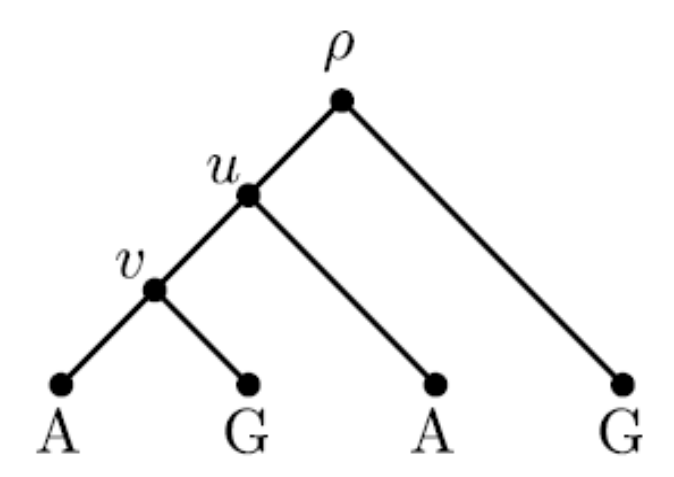
\includegraphics[scale=0.25]{Bioinformatics_Problem_Sheet2_fig1.png}
		\end{figure}
	%\begin{enumerate}
		%%Fitch and Sankkoff has been taken out of the lecture, Sankoff is now called Small Parsimony Problem
		%%\item Use the Fitch algorithm to find the minimum parsimony cost for the given tree and identify the optimal state assignments for each node, which have the minimum cost. 
		%%\item Verify that we would also obtain the same minimum cost in part (a) by using the Sankoff algorithm with c(A; G) = 1 and c(A; A) = c(G; G) = 0. 
		%%\item What are the optimal state assignments you would obtain from part (b)? Are there any discrepancies with those you found in part (a)? If there are, provide an explanation. 
	%\end{enumerate}
	\item Given the following distance matrix, calculate an evolutionary tree using UPGMA:
		\begin{table}[H]
		\centering
		\begin{tabular}{|l|r|r|r|l|l|l|}
		\hline
		 & \multicolumn{1}{l|}{A} & \multicolumn{1}{l|}{B} & \multicolumn{1}{l|}{C} & D & E & F \\ \hline
		A & 0 & \multicolumn{1}{l|}{} & \multicolumn{1}{l|}{} &  &  &  \\ \hline
		B & 2 & 0 & \multicolumn{1}{l|}{} &  &  &  \\ \hline
		C & 4 & 4 & 0 &  &  &  \\ \hline
		D & 6 & 6 & 6 & \multicolumn{1}{r|}{0} &  &  \\ \hline
		E & 6 & 6 & 6 & \multicolumn{1}{r|}{4} & \multicolumn{1}{r|}{0} &  \\ \hline
		F & 8 & 8 & 8 & \multicolumn{1}{r|}{8} & \multicolumn{1}{r|}{8} & \multicolumn{1}{r|}{0} \\ \hline
		\end{tabular}
		%%\caption{Distance Matrix}
		\label{}
		\end{table}
	\item  Given the following distance matrix, calculate an evolutionary tree using neighbour joining:
		\begin{table}[H]
		\centering
		\begin{tabular}{|l|r|r|r|l|l|}
		\hline
		 & \multicolumn{1}{l|}{A} & \multicolumn{1}{l|}{B} & \multicolumn{1}{l|}{C} & D & E \\ \hline
		A & 0 & \multicolumn{1}{l|}{} & \multicolumn{1}{l|}{} &  &  \\ \hline
		B & 5 & 0 & \multicolumn{1}{l|}{} &  &  \\ \hline
		C & 4 & 7 & 0 &  &  \\ \hline
		D & 7 & 10 & 7 & \multicolumn{1}{r|}{0} &  \\ \hline
		E & 6 & 9 & 6 & \multicolumn{1}{r|}{5} & \multicolumn{1}{r|}{0} \\ \hline
		\end{tabular}
		%%\caption{Distance Matrix}
		\label{}
		\end{table}
\end{enumerate}

\textbf{Optional task} Feel free to complete as much as you feel confident. 
One of the most popular programming langage in bioinformatics is R (\url{https://cran.r-project.org/}).

Try to run and understand the following code:

%\begin{lstlisting}
\begin{verbatim}
head(iris) #inspecting iris dataset
str(iris) #still inspecting
?help(iris)
dd <- dist(scale(iris[,-5]), method = "euclidean") #creating distance matrix
hc <- hclust(dd, method = "average") #UPGMA clustering
plot(hc)
\end{verbatim}
%\end{lstlisting}

\begin{enumerate}
\item Familiarise yourself with the iris dataset (see code above) as well as distance metrices (help(dist)), could you think of any situations the euclidean distance is not appropriate?
\item Familiarise yourself with the hirachical clustering function (help(hclust)).
\item Familiarise yourself with cutree (help(cutree)). Whats the point of this function? 

\begin{enumerate}
\item Investigate the 3 cluster solution (table(cutree(hc,3))).
\item Compare the 3 cluster solution with the actual classification (stored column 5). table(cutree(hc,3), iris[,5]). 
\item How do you interpret this table? Is this result expected? 
\item Would it improve if you took the 4 cluster solution instead? How about using the default Ward clustering instead UPGMA?
\end{enumerate}

\item Try to write code to compute the euclidean distances yourself
\item Very optional: try to write code to perform UPGMA clustering yourself and run it on the distance matrix dd.
\end{enumerate}

\end{document}
